\documentclass[12pt,a4paper,titlepage]{report}
\usepackage[utf8]{inputenc}
\usepackage[T1]{fontenc}
\usepackage{amsmath}
\usepackage{amsfonts}
\usepackage{amssymb}
\usepackage{graphicx}
\usepackage{changepage} 
\usepackage{systeme}
\usepackage{mathtools}
\usepackage{booktabs}
\usepackage[margin=1in]{geometry}

\newcommand\setItemnumber[1]{\setcounter{enumi}{\numexpr#1-1\relax}}
\newcommand{\R}{\mathbb{R}}
\newcommand{\N}{\mathbb{N}}
\newcommand{\C}{\mathbb{C}}
\title{Math 360 - Project 1: Symbiosis (Mutualism)}
\author{Ethan Rahman}

\begin{document}
	\maketitle
	\pagebreak
	\section*{Problem 1}
		Honey bees and clover plants have a symbiotic relationship that is mutually beneficial. The assigned problem attempts to model this relationship using a non-linear dynamical system. The model variables are defined in table 1 below.
	
		\begin{table}[ht]
			\centering
			\begin{tabular}{ccccc}
				\toprule
				Variable & Description \\ 
				\midrule 
				\(n\) & Number of years since 1990 \\ 
				\(X_{n}\) & Population of bees at year \(n\) \\
				\(Y_{n}\) & Population of clover plants at year \(n\) \\ 
				\(\Delta X_{n}\) & Net change in bee population during year \(n\) \\
				\(\Delta Y_{n}\) & Net change in clover plant population during year \(n\)   \\ 
				\(a\) & Proportionality constant for death rate of bees \\ 
				\(b\) & Proportionality constant for birth rate of bees  \\ 
				\(c\) & Proportionality constant for death rate of clover plants  \\ 
				\(d\) & Proportionality constant for birth rate of bees  \\ 
				\bottomrule
			\end{tabular}
			\caption{Definition of all variables used in this paper.}
		\end{table}
		The exact model is essentially the sum of two terms for each population. The first term in both models can be thought of as the death rate function: \(-aX_{n}\) for bees and \(-cY_{n}\) for clovers. More organism will die just by random chance or aging even the population of that organism is higher. The parameters \(a\) and \(c\) represent proportionality constants for the death function in both populations. And because they decrease the population, the sign of the terms are negative. Because bees and clovers have a mutually beneficial relationship we wouldn't expect there to be any interaction effects here. \\
		
		The second term is the birth rate function: \(bX_{n}Y_{n}\) for bees and \(dX_{n}Y_{n}\) for clover plants. Here is where the interaction effects become relevant. Bees benefit from having a higher population of clover plants because they can use feed on more of their nectar. Simultaneously, clover plants benefit from having a higher population of bees because there is a greater chance each bee will spread more pollen. \(b\) and \(d\) represent proportionality constants for the birth function in both populations. \\
		
		Put together, the model is simply the sum of the death rate function and the birth rate function for each population: 
		\[\Delta X_{n} = -aX_{n} + b X_{n}Y_{n}\]
		\[\Delta Y_{n} = -cY_{n} + d X_{n}Y_{n}\]

	\section*{Problem 2}
		For the next section, we're looking at the model when the parameters in table 2 are specified along with the initial points \(X_{0} = 200\) and \(Y_{0} = 300\). 
		\begin{table}[ht]
			\centering
			\begin{tabular}{cl}
				\toprule
				Parameter & Value \\ 
				\midrule 
				\(a\) & 0.2\\ 
				\(b\) & 0.001 \\
				\(c\) & 0.3  \\ 
				\(d\) & 0.002  \\ 
				\bottomrule
			\end{tabular}
			\caption{Set of values for each parameter}
			\label{params1}
		\end{table}
		The results of the model are recorded in table \ref{tab:p2}. For the year 1998, the population of bees is 7,475 while the population of clovers is 14,360. The population of both organisms quickly grows and becomes too large to calculate using Python by the year 2007! So we are unable to provide an answer for the population in the year 2008 but the long run behavior of the model using this set of parameters is clear. The population becomes infinitely large without reaching an equilibrium. 
		\begin{table} 
			\centering
			\begin{tabular}{lrrrr}
\toprule
{} &      \(X\) &      \(Y\) & \(\Delta X\) & \(\Delta Y\) \\
Year &            &            &              &              \\
\midrule
1990 &  2.000e+02 &  3.000e+02 &    2.000e+01 &    3.000e+01 \\
1991 &  2.200e+02 &  3.300e+02 &    2.860e+01 &    4.620e+01 \\
1992 &  2.486e+02 &  3.762e+02 &    4.380e+01 &    7.419e+01 \\
1993 &  2.924e+02 &  4.504e+02 &    7.321e+01 &    1.283e+02 \\
1994 &  3.656e+02 &  5.787e+02 &    1.384e+02 &    2.495e+02 \\
1995 &  5.041e+02 &  8.282e+02 &    3.167e+02 &    5.865e+02 \\
1996 &  8.207e+02 &  1.415e+03 &    9.969e+02 &    1.898e+03 \\
1997 &  1.818e+03 &  3.312e+03 &    5.657e+03 &    1.105e+04 \\
1998 &  7.475e+03 &  1.436e+04 &    1.058e+05 &    2.104e+05 \\
1999 &  1.133e+05 &  2.247e+05 &    2.544e+07 &    5.086e+07 \\
2000 &  2.555e+07 &  5.108e+07 &    1.305e+12 &    2.611e+12 \\
2001 &  1.305e+12 &  2.611e+12 &    3.408e+21 &    6.816e+21 \\
2002 &  3.408e+21 &  6.816e+21 &    2.323e+40 &    4.646e+40 \\
2003 &  2.323e+40 &  4.646e+40 &    1.079e+78 &    2.158e+78 \\
2004 &  1.079e+78 &  2.158e+78 &   2.329e+153 &   4.659e+153 \\
2005 & 2.329e+153 & 4.659e+153 &   1.085e+304 &   2.170e+304 \\
2006 & 1.085e+304 & 2.170e+304 &          inf &          inf \\
2007 &        inf &        inf &          nan &          nan \\
2008 &        nan &        nan &          nan &          nan \\
\bottomrule
\end{tabular}

			\caption{The model values calculated using a Python script. An overflow error is thrown by the year 2006 for \(\Delta X\) and \(\Delta Y\).}
			\label{tab:p2}
		\end{table}
	\section*{Problem 3}
		For problem 3 we use the same parameters in table \ref{params1} but with initial values \(X_{0} = 100\) and \(Y_{0} = 150\). The results here are much more amenable to a visual representation. Figure \ref{fig:p3} depicts the model as a vector field with the specific path taken by the populations when they start at the given initial values.\\ 
		In 1998, the population of bees declines to 43 and the population of clovers is 42. By 2008 there are only 6 bees and 2 clovers. More specific values for the evolution of the population model are given in table \ref{tab:p3}. Over time it appears that both organisms go extinct. \\
		The model does not result in the populations being cut in half from the populations in table \ref{tab:p2} from problem 2. This is because the model is defined by non-linear difference equations. To illustrate this, set \(X_{n} = 2X_{n}\) and \(Y_{n} = 2Y_{n}\) in the birth functions for bees and clovers:
		\[X_{Birth} = b (2X_{n})(2Y_{n}) = 4bX_{n}Y_{n}\]
		\[Y_{Birth} = d (2X_{n})(2Y_{n}) = 4dX_{n}Y_{n}\]
		As you can see,  doubling the populations results in the birth rate increasing by a factor of 4 for both populations! That is, the birth function has increasing returns to scale and is non-linear. \\
		
		\begin{figure}[htbp]
			\centerline{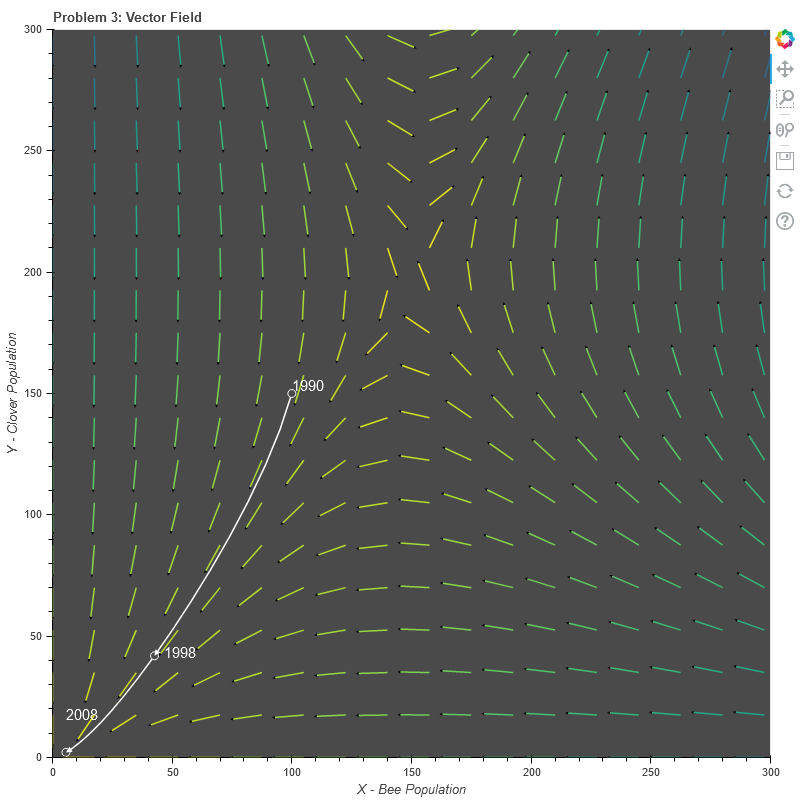
\includegraphics[scale=.5]{charts/problem3_chart.png}}
			\caption{The model is represented as a vector field. The lengths of each vector are kept the same, but the color of each vector is determined by the magnitude of the vector at that point. Light yellow vectors have the lowest magnitude and dark purple vectors have the largest. The white shows the evolution of the populations when the initial conditions are \(X_{0} = 100\) and \(Y_{0} = 150\) are chosen.}
			\label{fig:p3}
		\end{figure}
		At the same time, the death functions have constant returns to scale:
		\[X_{Death} = -a (2X_{n}) = -2aX_{n}\]
		\[Y_{Death} = -c (2Y_{n}) = -2cY_{n}\]
		As a result, the birth rate tends to increase faster than the death rate as the populations get larger. At the same time however, the death rate will decrease at a slower rate than the birth rate for decreasing populations. If both populations are declining, then generally speaking the death function will stay higher than the birth function in future years. If both populations are increasing, then the birth function will generally be larger than the death function. 
		\begin{table} 
			\centering
			\begin{tabular}{lrrrr}
\toprule
{} &  \(X\) &  \(Y\) & \(\Delta X\) & \(\Delta Y\) \\
Year &        &        &              &              \\
\midrule
1990 & 100.00 & 150.00 &        -5.00 &       -15.00 \\
1991 &  95.00 & 135.00 &        -6.18 &       -14.85 \\
1992 &  88.83 & 120.15 &        -7.09 &       -14.70 \\
1993 &  81.73 & 105.45 &        -7.73 &       -14.40 \\
1994 &  74.00 &  91.05 &        -8.06 &       -13.84 \\
1995 &  65.94 &  77.21 &        -8.10 &       -12.98 \\
1996 &  57.85 &  64.23 &        -7.85 &       -11.84 \\
1997 &  49.99 &  52.39 &        -7.38 &       -10.48 \\
1998 &  42.61 &  41.91 &        -6.74 &        -9.00 \\
1999 &  35.88 &  32.91 &        -5.99 &        -7.51 \\
2000 &  29.88 &  25.40 &        -5.22 &        -6.10 \\
2001 &  24.66 &  19.30 &        -4.46 &        -4.84 \\
2002 &  20.21 &  14.46 &        -3.75 &        -3.75 \\
2003 &  16.46 &  10.71 &        -3.12 &        -2.86 \\
2004 &  13.34 &   7.85 &        -2.56 &        -2.14 \\
2005 &  10.78 &   5.70 &        -2.09 &        -1.59 \\
2006 &   8.68 &   4.11 &        -1.70 &        -1.16 \\
2007 &   6.98 &   2.95 &        -1.38 &        -0.84 \\
2008 &   5.61 &   2.11 &        -1.11 &        -0.61 \\
\bottomrule
\end{tabular}

			\caption{The model evolution for the initial conditions \(X_{0} = 100\) and \(Y_{0} = 150\) given the parameters in table \ref{params1}.}
			\label{tab:p3}
		\end{table}
		This can help explain why small changes in the initial condition of the populations can result in very different long term behaviors - the starting conditions basically determine whether the death function will be larger or smaller than the birth function very early on. And consistent with this description, the vector field in \ref{fig:p3} can give us an idea of which points result in growing populations and declining populations. 
		
\end{document}